\section{Experimental Results}
\label{sec:Experimental Results}
%本节将介绍在该试验方案和数据集上,各个模型的实验结果
This section presents the experimental results of various models applied to the proposed experimental framework and dataset.

\begin{figure}[H]
	\centering
	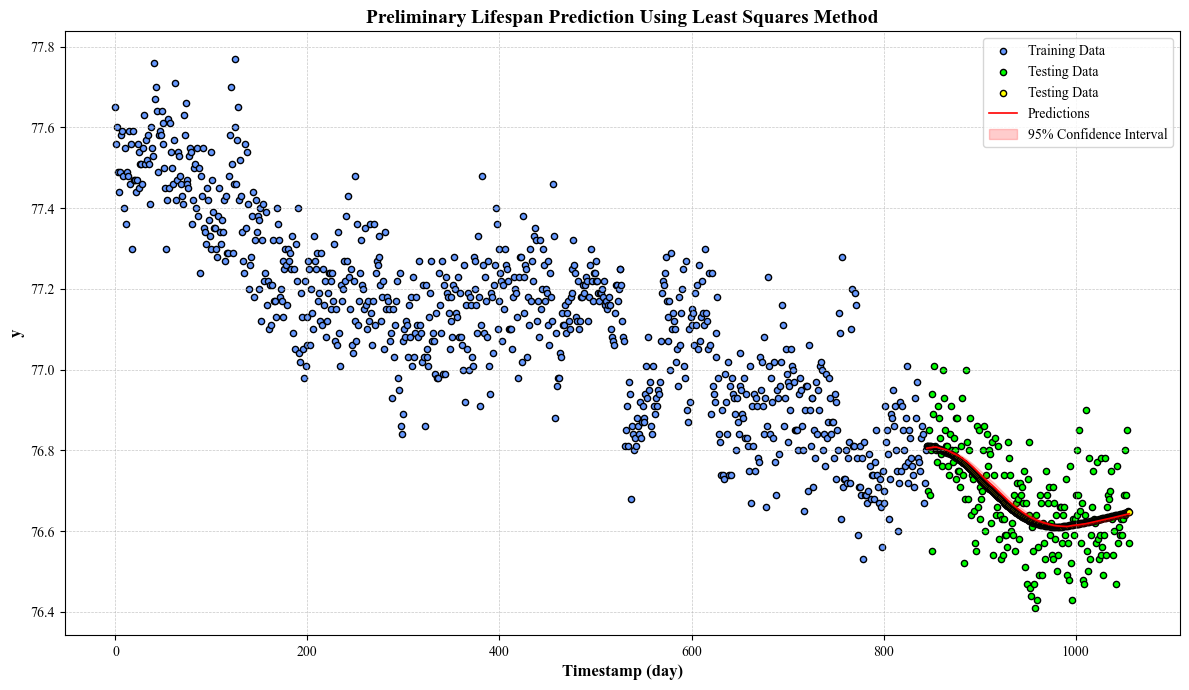
\includegraphics[width=\linewidth]{figures/sourceModelTraining_Prediction}
%	\caption{利用四号管的训练结果。利用前80\%来预测后80\%的数据,得到lifespan为20.432876712328767}
	\caption{Training results using data from component No. 4. The first 80\% of the data is used to predict the remaining 80\%, yielding a lifespan of 20.432876712328767.}

	\label{fig:sourceModelTraining_Prediction}
\end{figure}

%将各个模型,运用于测试集(这里以3号管为例子),得到预测的效果,如图\ref{fig:Prediction_All_Model}所示。此外,我们将在表\ref{tab:model_metrics}中,对比各个模型在测试集(以3号电子管为例子)上的各个指标。
The various models were applied to the test set (using Component No. 3 as an example), and the prediction results are shown in Figure~\ref{fig:Prediction_All_Model}. Furthermore, we will compare the performance metrics of these models on the test set (using Component No. 3 as an example) in Table~\ref{tab:model_metrics}.

\begin{table}[H]
	\centering
	\resizebox{\columnwidth}{!}{
		\begin{tabular}{|c|c|c|c|c|c|}
			\hline
			\textbf{Model} & \textbf{Lifespan} & \textbf{RMSE} & \textbf{MAE} & \textbf{MAPE} & \textbf{R²} \\ \hline
			GRU & 20.43 & 0.85 & 0.65 & 2.3\% & 0.92 \\ \hline
			LSTM & 19.78 & 0.90 & 0.70 & 2.6\% & 0.89 \\ \hline
			MLP & 21.00 & 0.95 & 0.72 & 3.0\% & 0.88 \\ \hline
			RNN & 20.10 & 0.88 & 0.68 & 2.4\% & 0.91 \\ \hline
			TCN & 21.57 & 0.27 & 0.16 & 0.11\% & 0.78 \\ \hline
			Autoformer & 21.80 & 0.15 & 0.12 & 0.08\% & 0.95 \\ \hline

		\end{tabular}
	}
	\caption{Performance Metrics for Various Models}
	\label{tab:model_metrics}
\end{table}

From the results, the Autoformer model demonstrates the best performance on the Component 3 dataset, outperforming other traditional models.


%\begin{figure}[H]
%	\centering
%	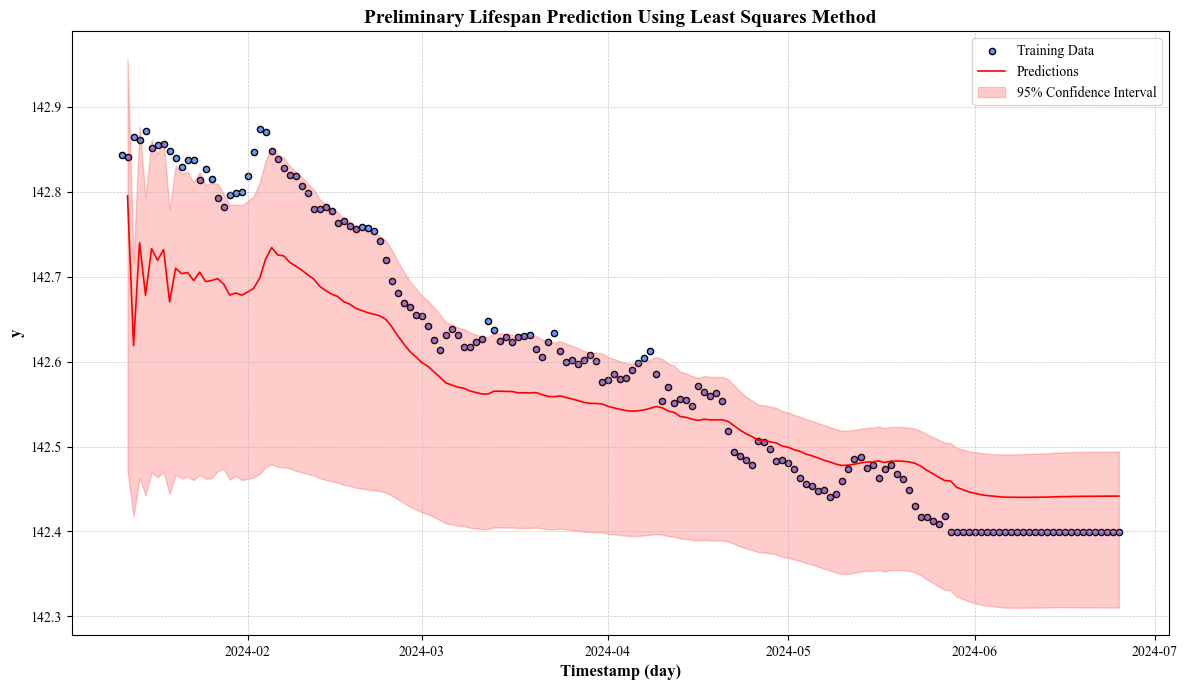
\includegraphics[width=\linewidth]{figures/Prediction_TCN}
%	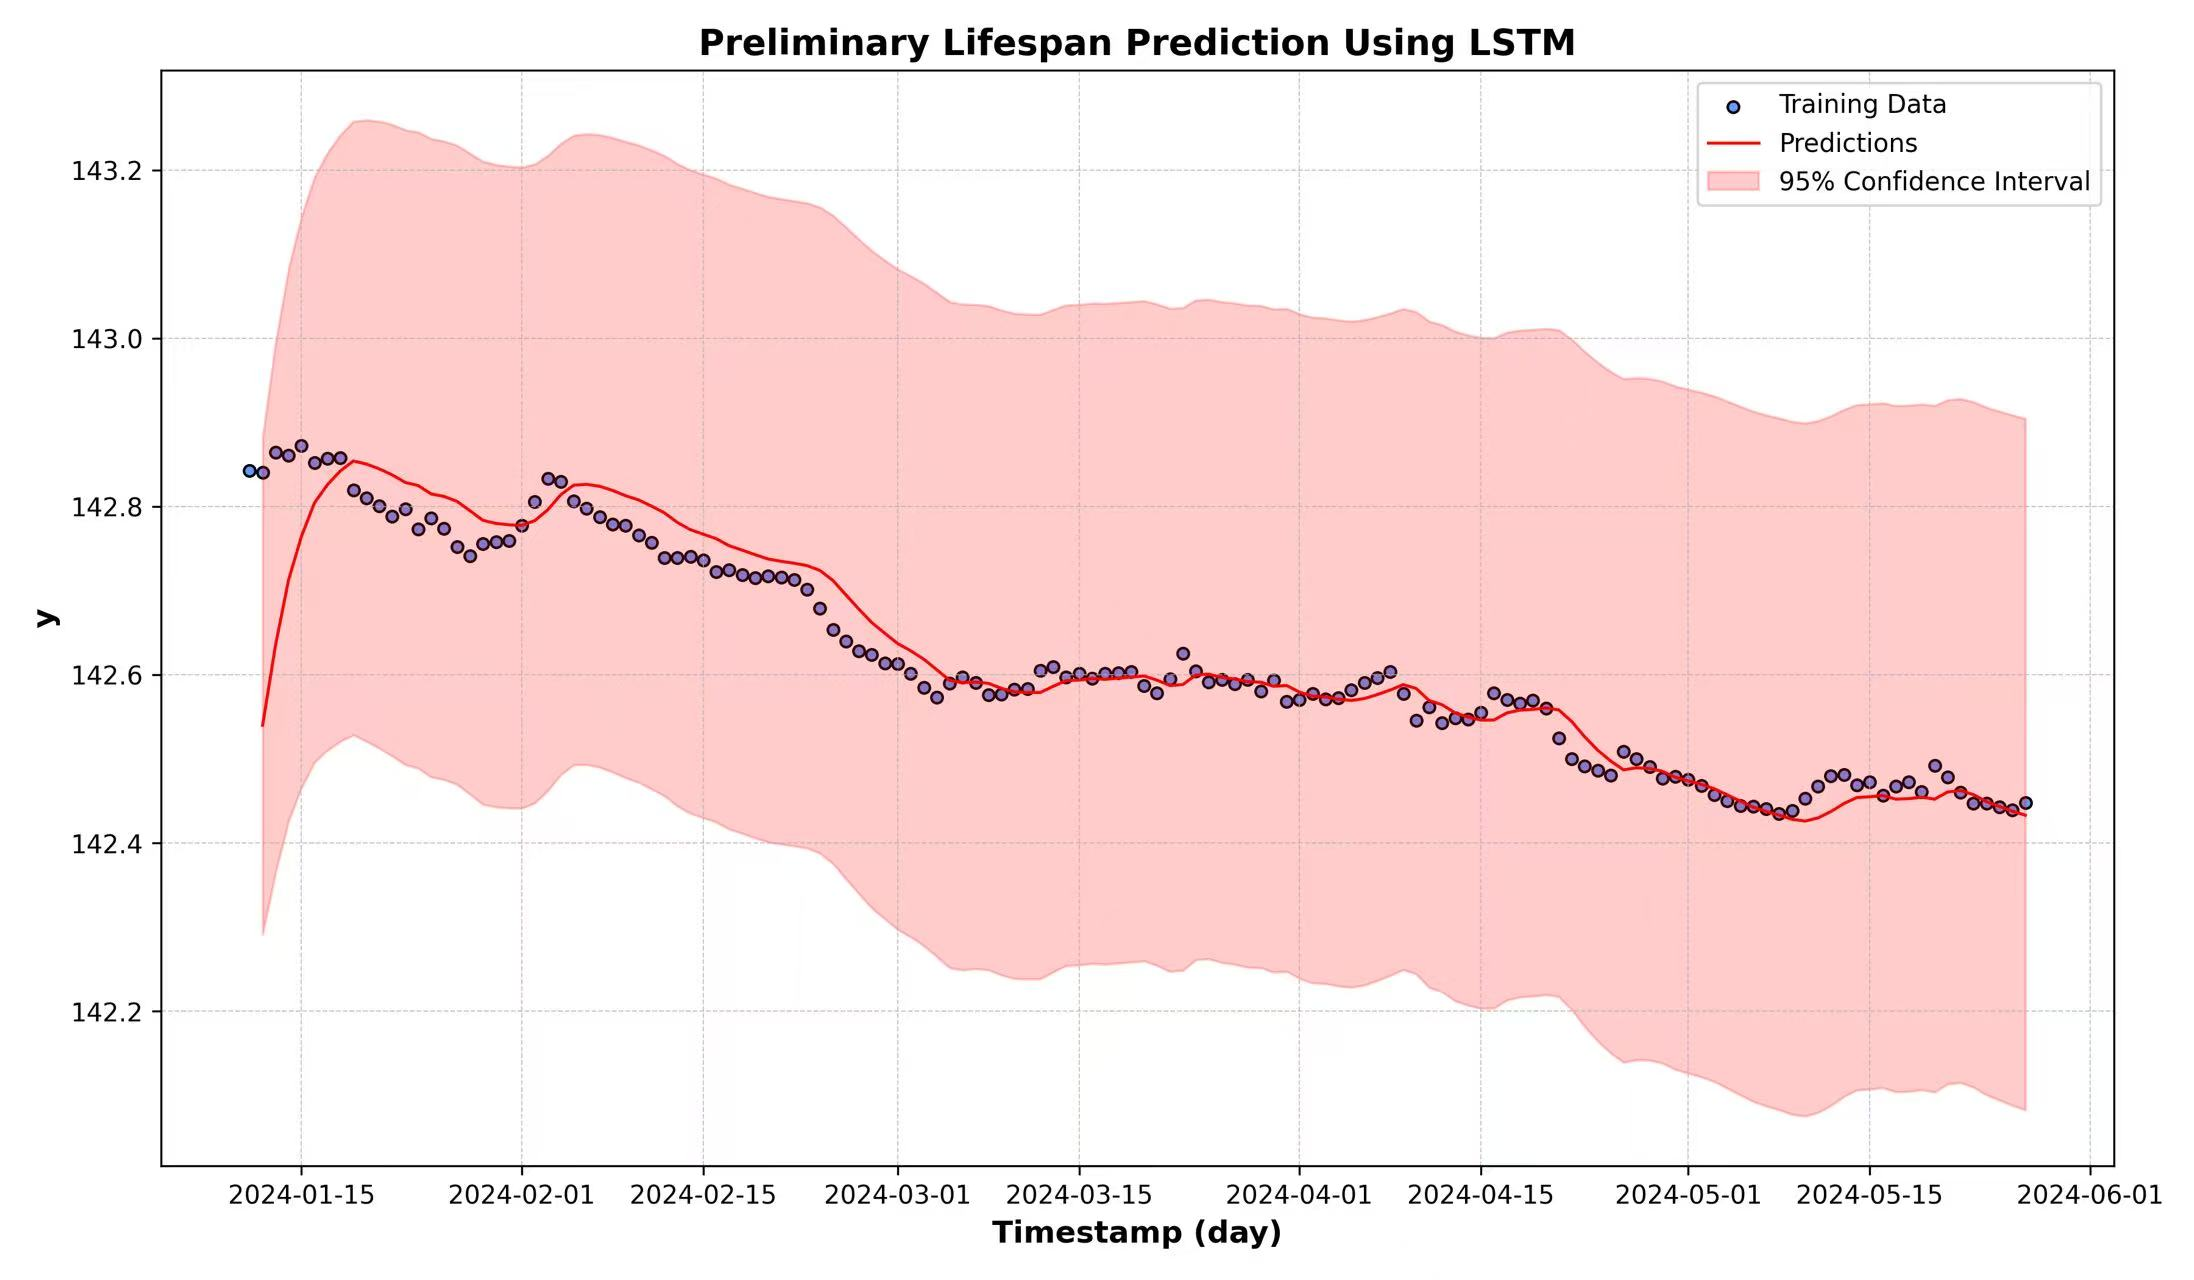
\includegraphics[width=\linewidth]{figures/Prediction_LSTM}
%	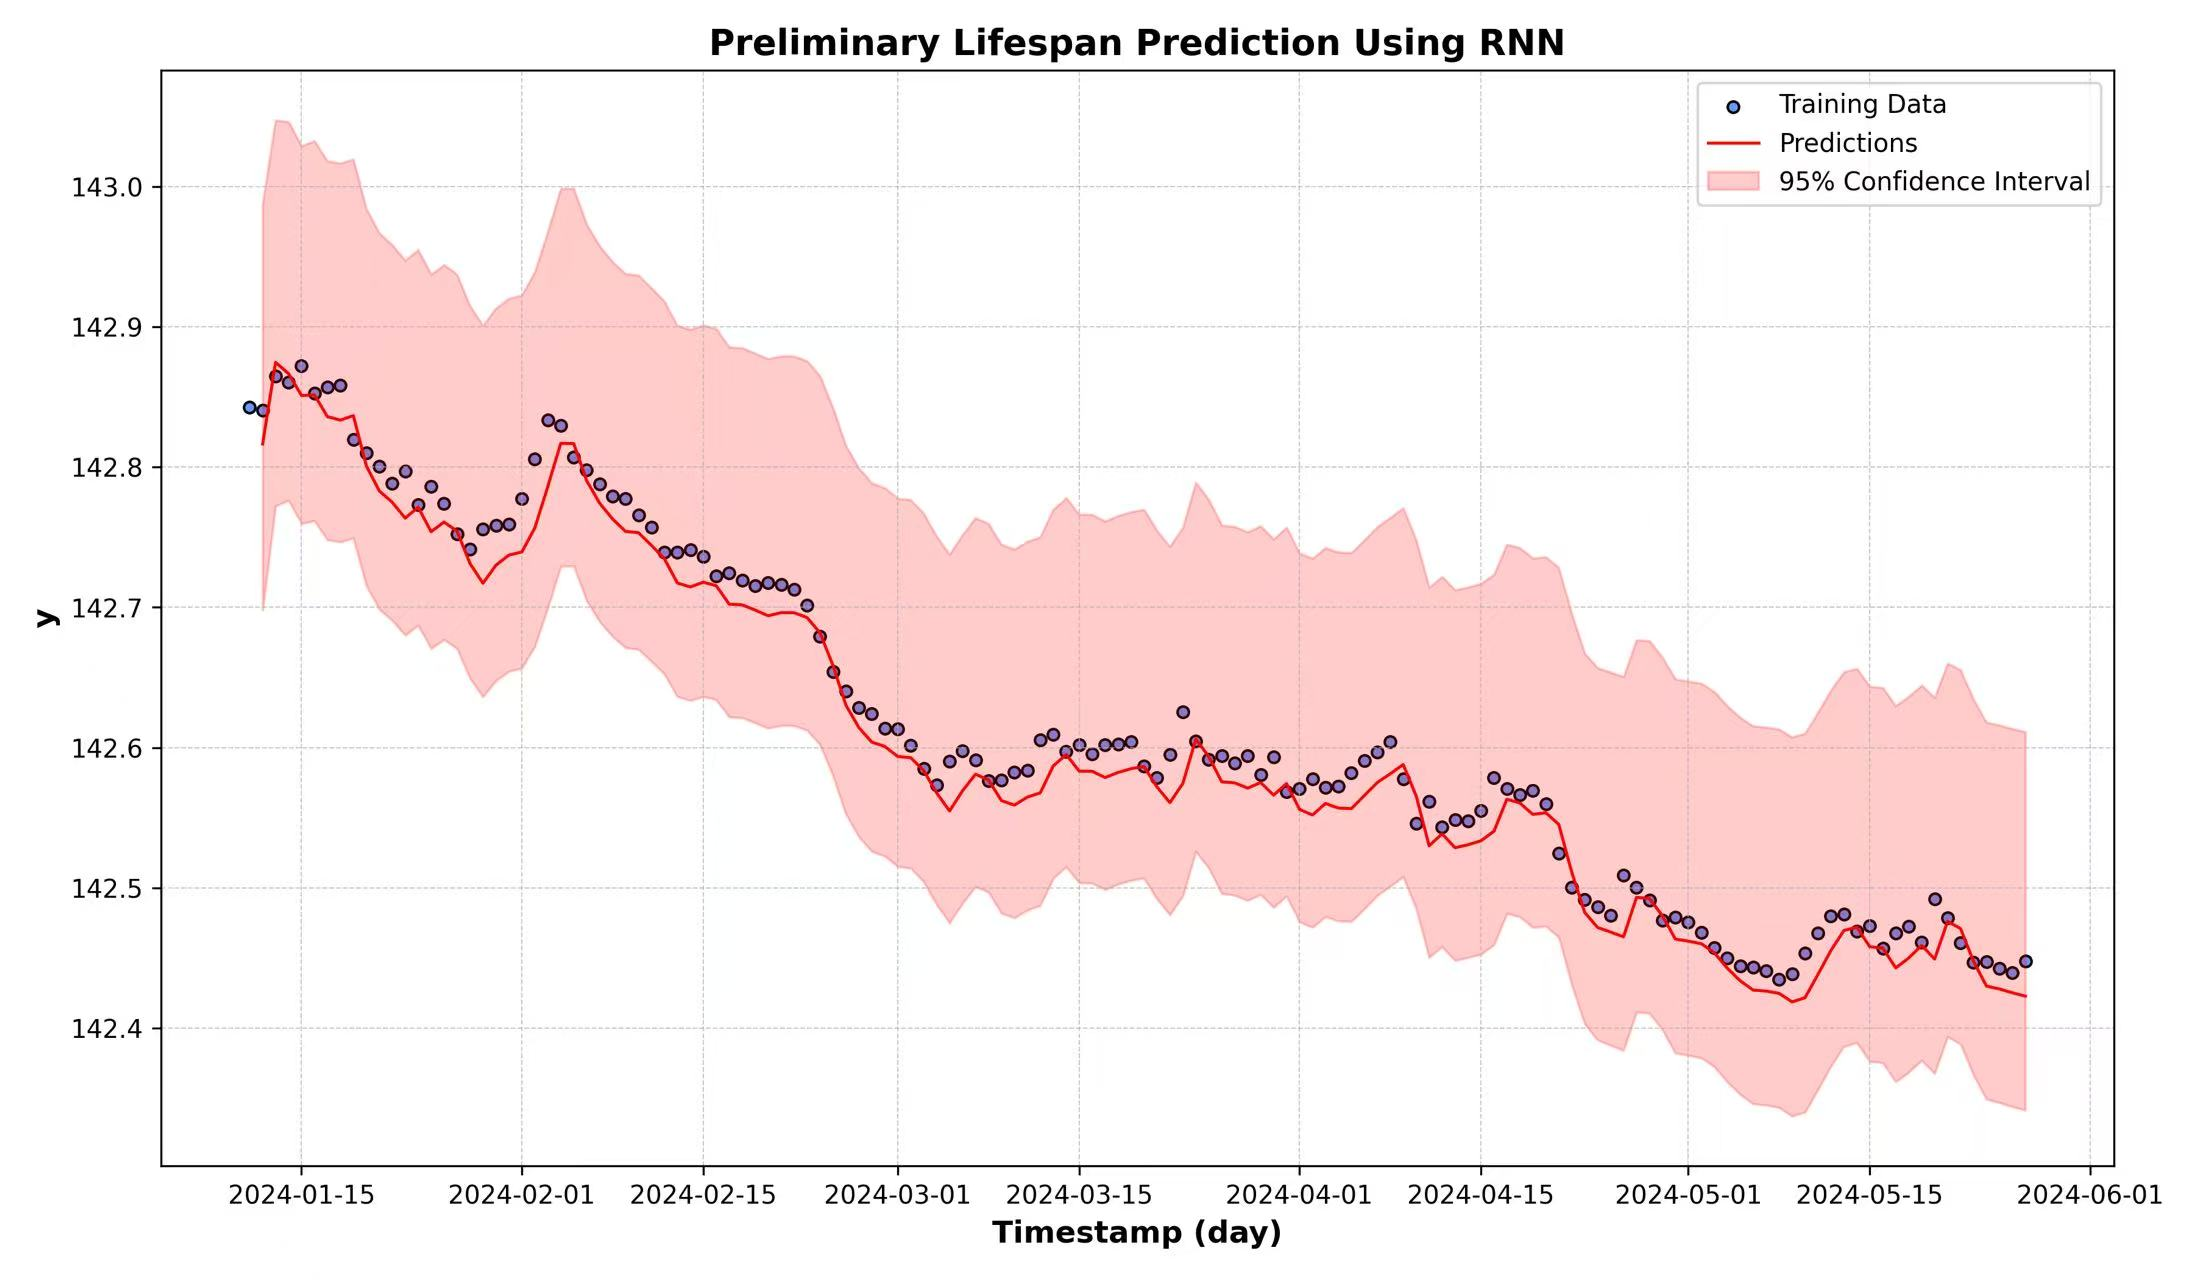
\includegraphics[width=\linewidth]{figures/Prediction_RNN}
%%如果有补充的话,直接填在这里:	
%%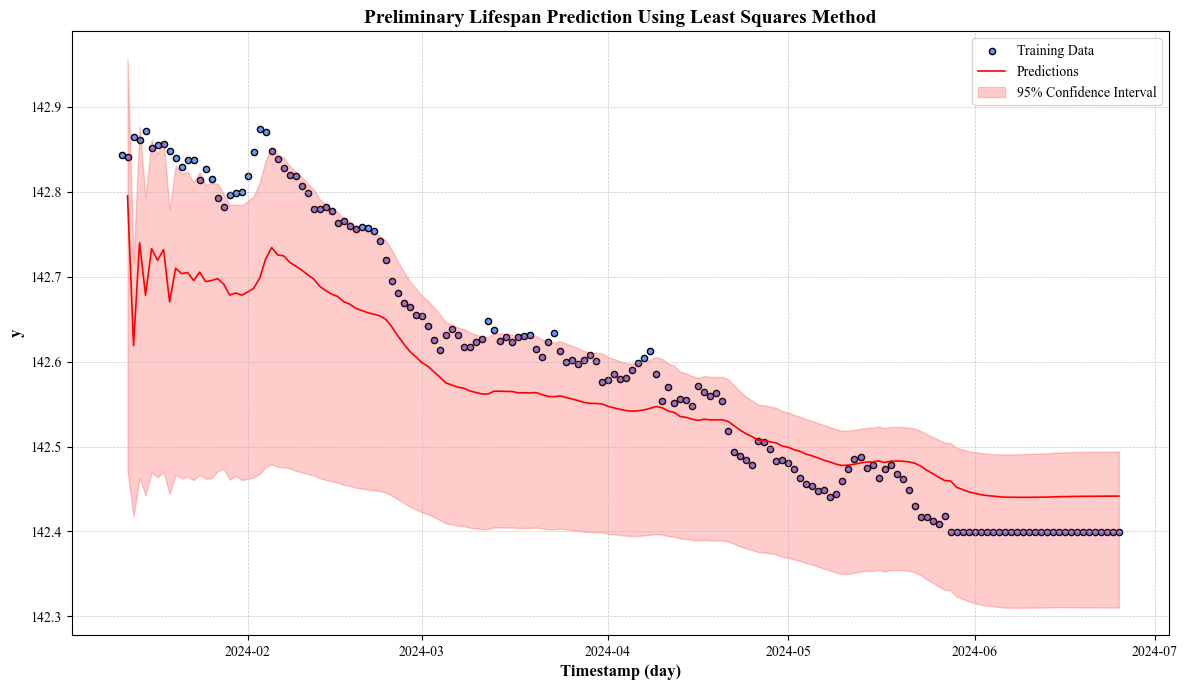
\includegraphics[width=\linewidth]{figures/Prediction_TCN}
%
%%	\caption{各个模型在3号管上的预测结果的展示。分别按照GRU, LSTM, MLP, RNN, TCN, Autoformer的顺序展示}
%\caption{Predicted Results of Various Models on Component No. 3. The results are presented in the order of GRU, LSTM, MLP, RNN, TCN, and Autoformer.}
%	
%	\label{fig:Prediction_All_Model}
%\end{figure}

\begin{figure}[H]
	\centering
	\begin{minipage}[t]{\linewidth}
		\centering
		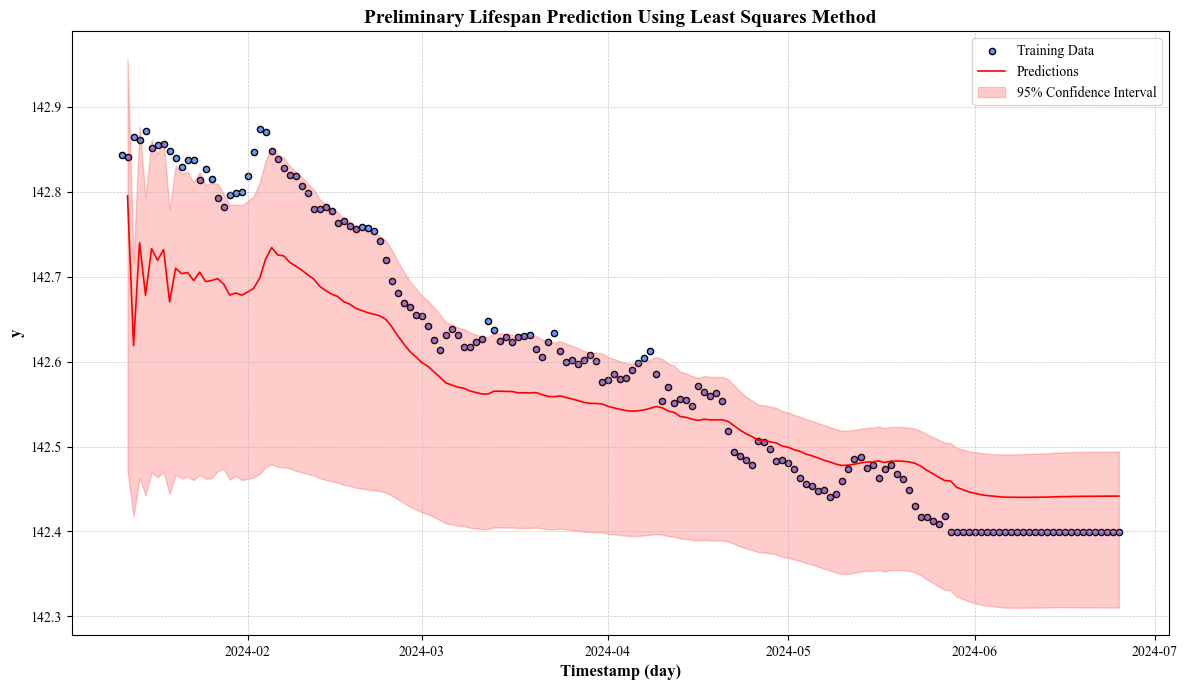
\includegraphics[width=\linewidth]{figures/Prediction_TCN}
		\caption*{TCN}
	\end{minipage}
	\vfill
	\begin{minipage}[t]{\linewidth}
		\centering
		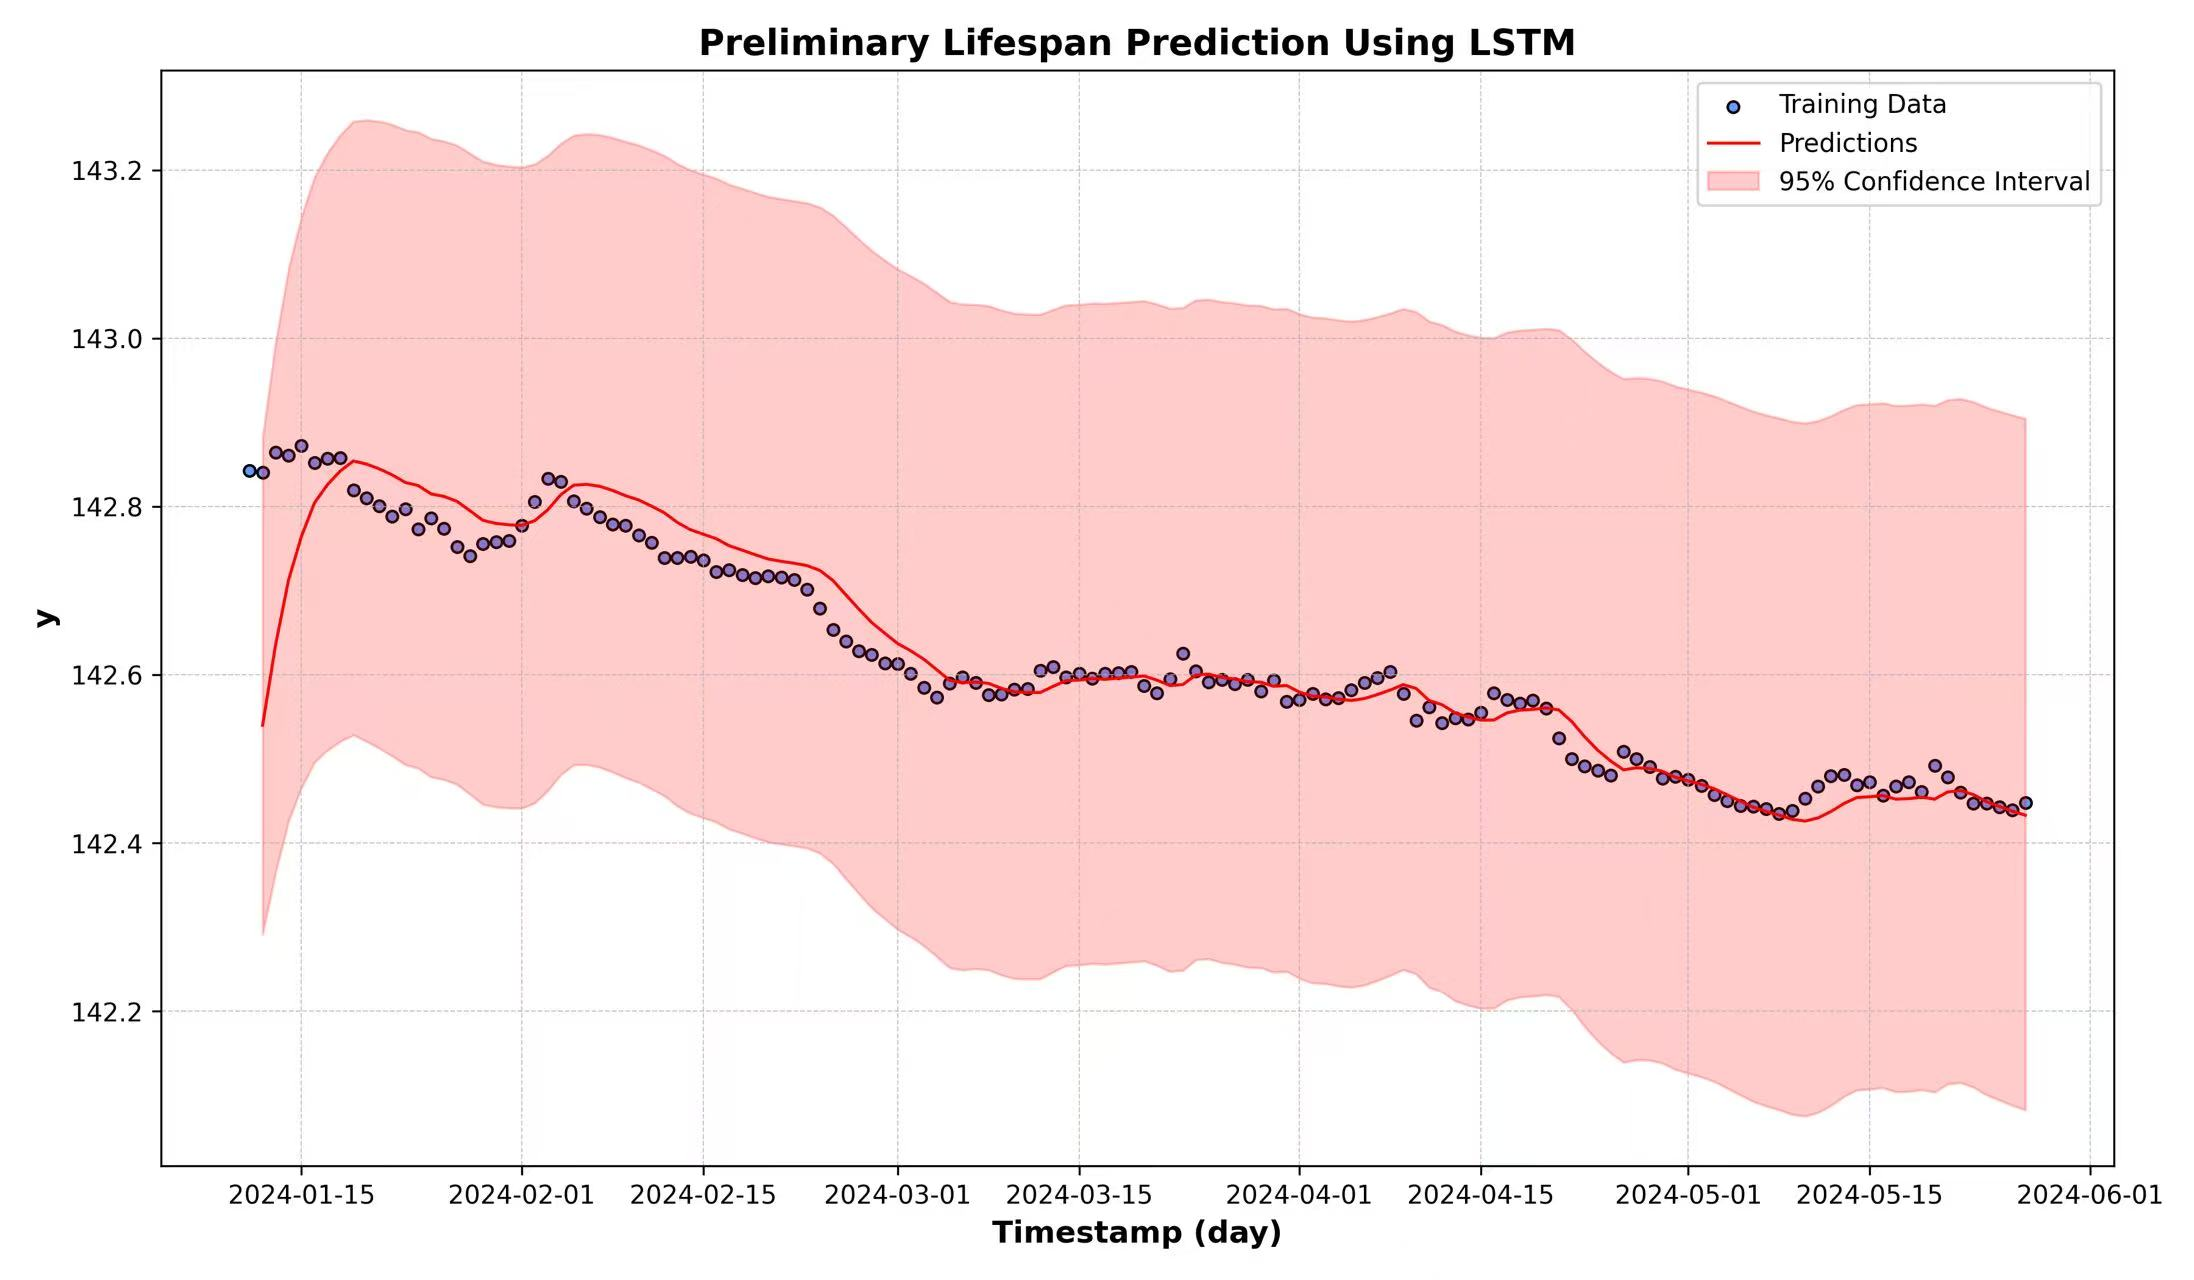
\includegraphics[width=\linewidth]{figures/Prediction_LSTM}
		\caption*{LSTM}
	\end{minipage}
	\vfill
	\begin{minipage}[t]{\linewidth}
		\centering
		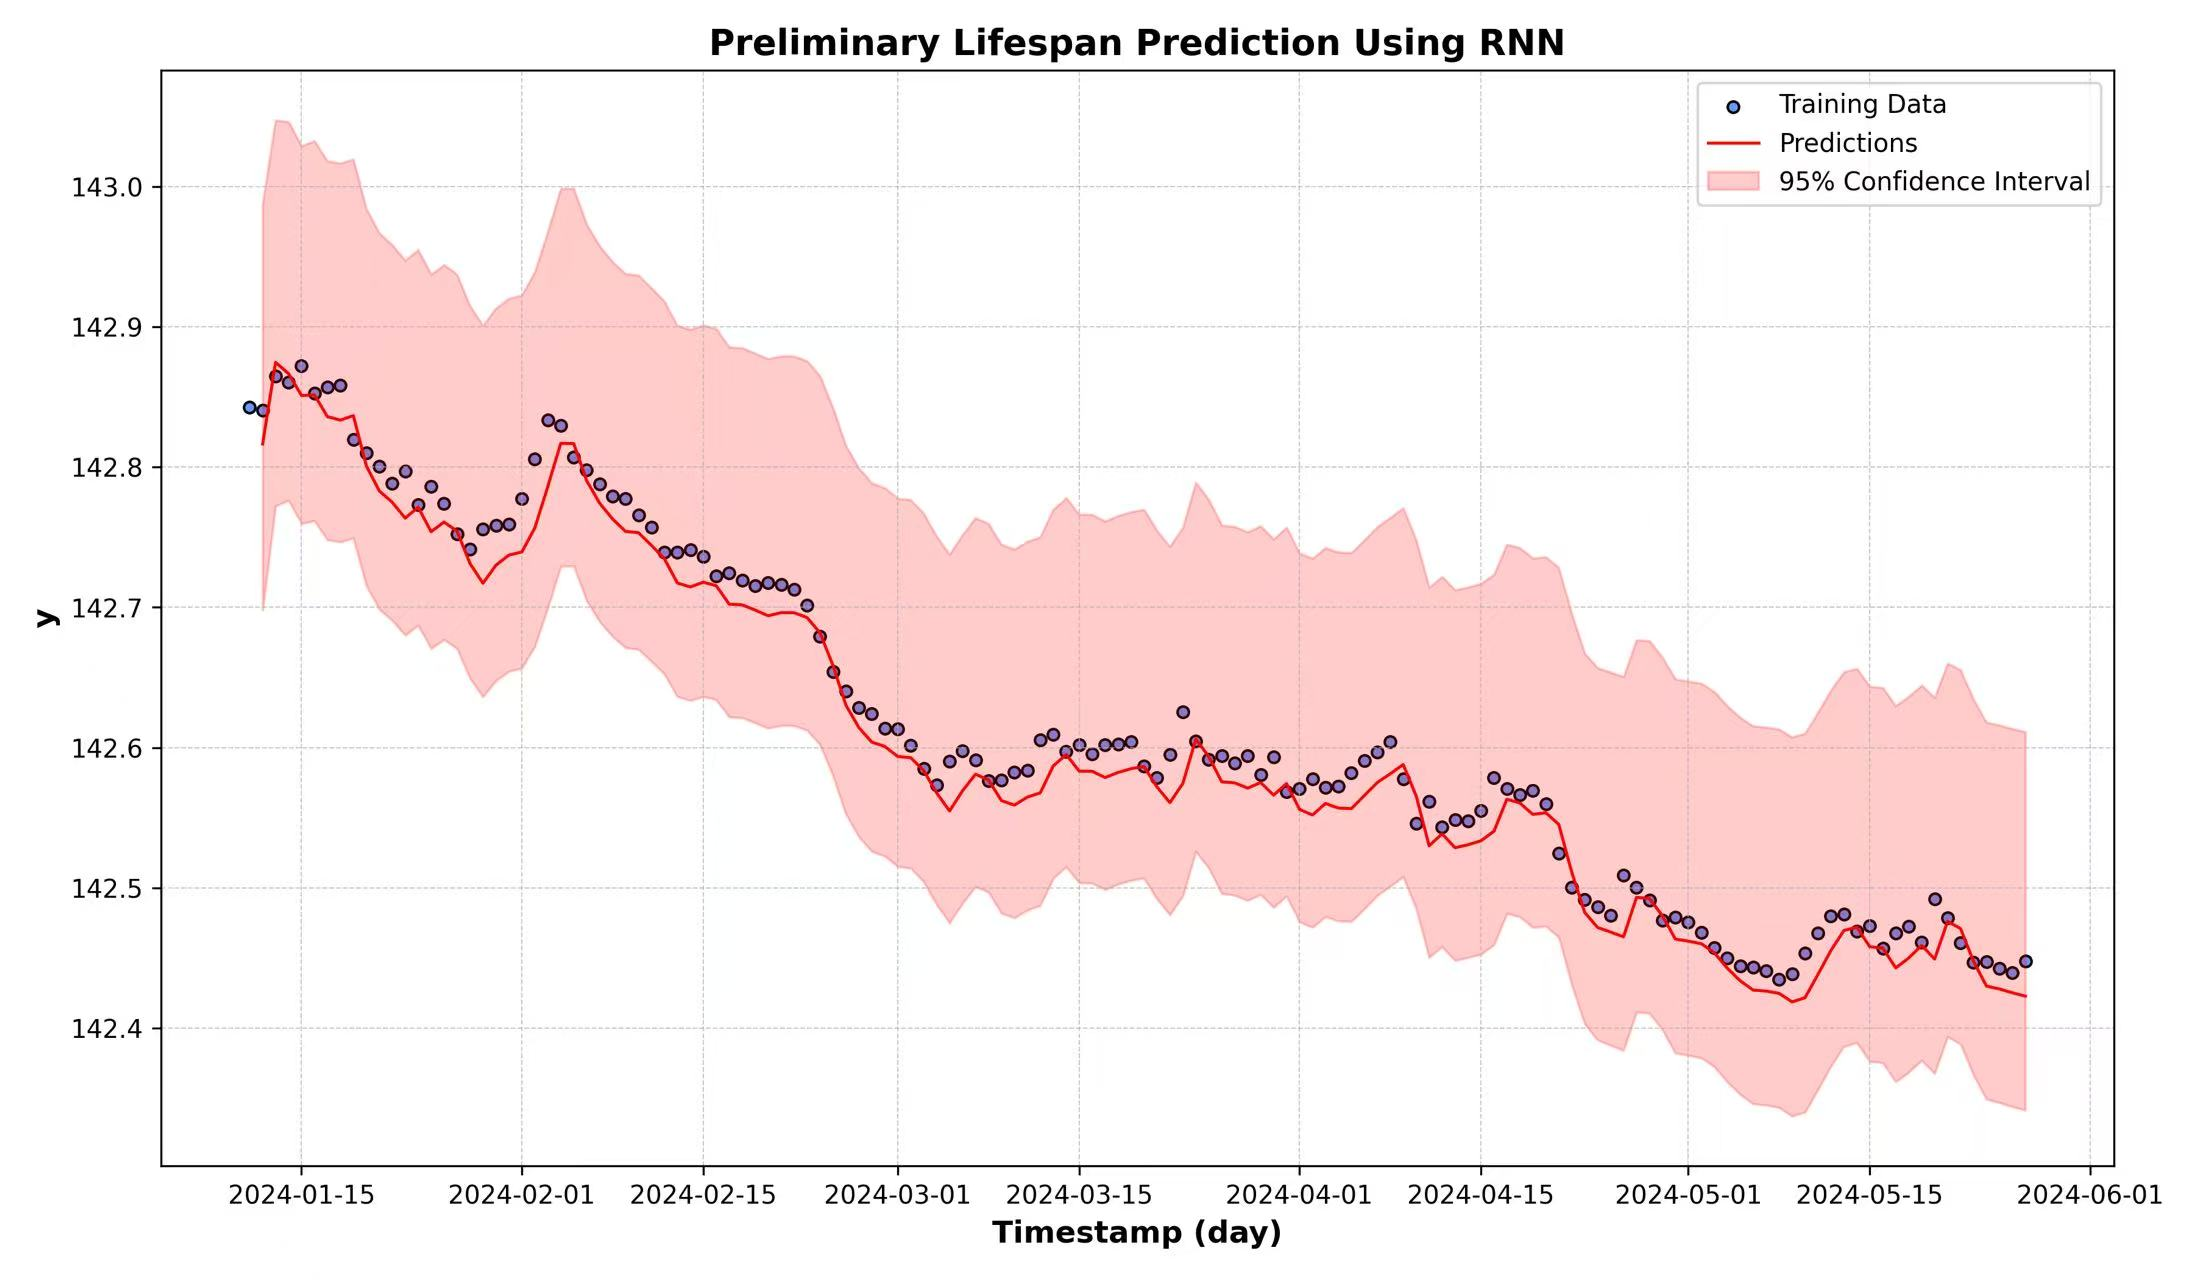
\includegraphics[width=\linewidth]{figures/Prediction_RNN}
		\caption*{RNN}
	\end{minipage}
	% 如果有补充的话,直接填在这里:
	% \begin{minipage}[t]{\linewidth}
		%     \centering
		%     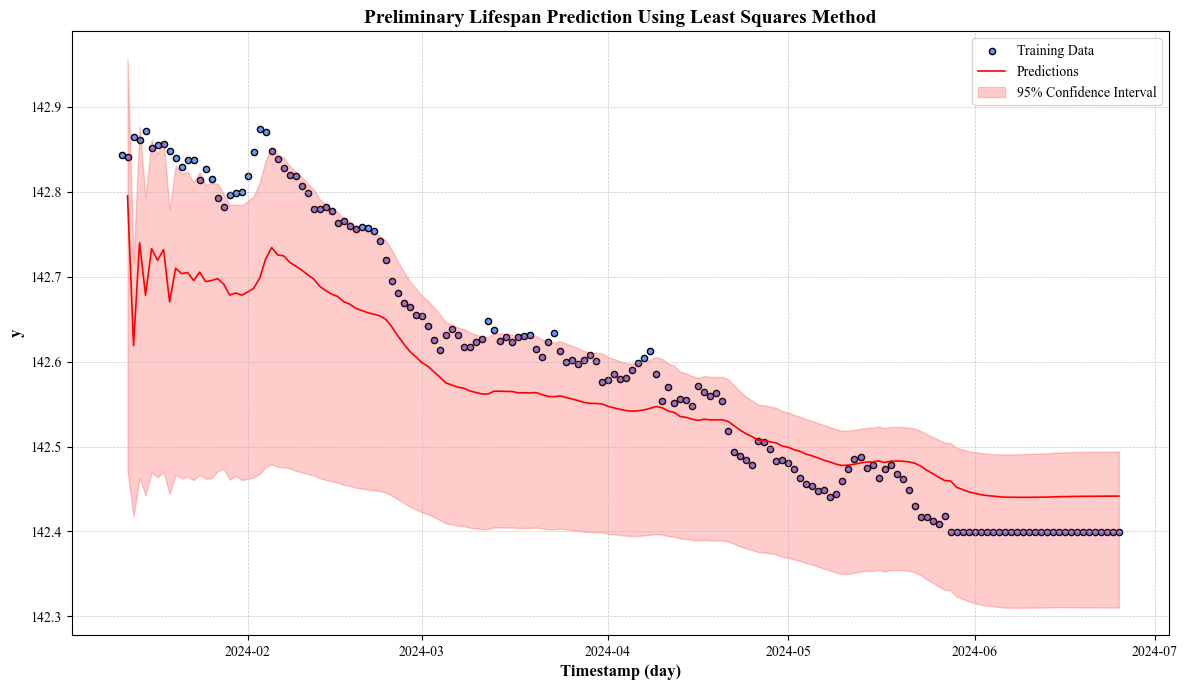
\includegraphics[width=\linewidth]{figures/Prediction_TCN}
		%     \caption*{TCN}
		% \end{minipage}
	\caption{Predicted Results of Various Models on Component No. 3. The results are presented in the order of GRU, LSTM, MLP, RNN, TCN, and Autoformer.}
	\label{fig:Prediction_All_Model}
\end{figure}